\documentclass[]{article}
\usepackage{lmodern}
\usepackage{amssymb,amsmath}
\usepackage{ifxetex,ifluatex}
\usepackage{fixltx2e} % provides \textsubscript
\ifnum 0\ifxetex 1\fi\ifluatex 1\fi=0 % if pdftex
  \usepackage[T1]{fontenc}
  \usepackage[utf8]{inputenc}
\else % if luatex or xelatex
  \ifxetex
    \usepackage{mathspec}
  \else
    \usepackage{fontspec}
  \fi
  \defaultfontfeatures{Ligatures=TeX,Scale=MatchLowercase}
\fi
% use upquote if available, for straight quotes in verbatim environments
\IfFileExists{upquote.sty}{\usepackage{upquote}}{}
% use microtype if available
\IfFileExists{microtype.sty}{%
\usepackage{microtype}
\UseMicrotypeSet[protrusion]{basicmath} % disable protrusion for tt fonts
}{}
\usepackage[margin=1in]{geometry}
\usepackage{hyperref}
\hypersetup{unicode=true,
            pdfborder={0 0 0},
            breaklinks=true}
\urlstyle{same}  % don't use monospace font for urls
\usepackage{color}
\usepackage{fancyvrb}
\newcommand{\VerbBar}{|}
\newcommand{\VERB}{\Verb[commandchars=\\\{\}]}
\DefineVerbatimEnvironment{Highlighting}{Verbatim}{commandchars=\\\{\}}
% Add ',fontsize=\small' for more characters per line
\usepackage{framed}
\definecolor{shadecolor}{RGB}{248,248,248}
\newenvironment{Shaded}{\begin{snugshade}}{\end{snugshade}}
\newcommand{\KeywordTok}[1]{\textcolor[rgb]{0.13,0.29,0.53}{\textbf{#1}}}
\newcommand{\DataTypeTok}[1]{\textcolor[rgb]{0.13,0.29,0.53}{#1}}
\newcommand{\DecValTok}[1]{\textcolor[rgb]{0.00,0.00,0.81}{#1}}
\newcommand{\BaseNTok}[1]{\textcolor[rgb]{0.00,0.00,0.81}{#1}}
\newcommand{\FloatTok}[1]{\textcolor[rgb]{0.00,0.00,0.81}{#1}}
\newcommand{\ConstantTok}[1]{\textcolor[rgb]{0.00,0.00,0.00}{#1}}
\newcommand{\CharTok}[1]{\textcolor[rgb]{0.31,0.60,0.02}{#1}}
\newcommand{\SpecialCharTok}[1]{\textcolor[rgb]{0.00,0.00,0.00}{#1}}
\newcommand{\StringTok}[1]{\textcolor[rgb]{0.31,0.60,0.02}{#1}}
\newcommand{\VerbatimStringTok}[1]{\textcolor[rgb]{0.31,0.60,0.02}{#1}}
\newcommand{\SpecialStringTok}[1]{\textcolor[rgb]{0.31,0.60,0.02}{#1}}
\newcommand{\ImportTok}[1]{#1}
\newcommand{\CommentTok}[1]{\textcolor[rgb]{0.56,0.35,0.01}{\textit{#1}}}
\newcommand{\DocumentationTok}[1]{\textcolor[rgb]{0.56,0.35,0.01}{\textbf{\textit{#1}}}}
\newcommand{\AnnotationTok}[1]{\textcolor[rgb]{0.56,0.35,0.01}{\textbf{\textit{#1}}}}
\newcommand{\CommentVarTok}[1]{\textcolor[rgb]{0.56,0.35,0.01}{\textbf{\textit{#1}}}}
\newcommand{\OtherTok}[1]{\textcolor[rgb]{0.56,0.35,0.01}{#1}}
\newcommand{\FunctionTok}[1]{\textcolor[rgb]{0.00,0.00,0.00}{#1}}
\newcommand{\VariableTok}[1]{\textcolor[rgb]{0.00,0.00,0.00}{#1}}
\newcommand{\ControlFlowTok}[1]{\textcolor[rgb]{0.13,0.29,0.53}{\textbf{#1}}}
\newcommand{\OperatorTok}[1]{\textcolor[rgb]{0.81,0.36,0.00}{\textbf{#1}}}
\newcommand{\BuiltInTok}[1]{#1}
\newcommand{\ExtensionTok}[1]{#1}
\newcommand{\PreprocessorTok}[1]{\textcolor[rgb]{0.56,0.35,0.01}{\textit{#1}}}
\newcommand{\AttributeTok}[1]{\textcolor[rgb]{0.77,0.63,0.00}{#1}}
\newcommand{\RegionMarkerTok}[1]{#1}
\newcommand{\InformationTok}[1]{\textcolor[rgb]{0.56,0.35,0.01}{\textbf{\textit{#1}}}}
\newcommand{\WarningTok}[1]{\textcolor[rgb]{0.56,0.35,0.01}{\textbf{\textit{#1}}}}
\newcommand{\AlertTok}[1]{\textcolor[rgb]{0.94,0.16,0.16}{#1}}
\newcommand{\ErrorTok}[1]{\textcolor[rgb]{0.64,0.00,0.00}{\textbf{#1}}}
\newcommand{\NormalTok}[1]{#1}
\usepackage{graphicx,grffile}
\makeatletter
\def\maxwidth{\ifdim\Gin@nat@width>\linewidth\linewidth\else\Gin@nat@width\fi}
\def\maxheight{\ifdim\Gin@nat@height>\textheight\textheight\else\Gin@nat@height\fi}
\makeatother
% Scale images if necessary, so that they will not overflow the page
% margins by default, and it is still possible to overwrite the defaults
% using explicit options in \includegraphics[width, height, ...]{}
\setkeys{Gin}{width=\maxwidth,height=\maxheight,keepaspectratio}
\IfFileExists{parskip.sty}{%
\usepackage{parskip}
}{% else
\setlength{\parindent}{0pt}
\setlength{\parskip}{6pt plus 2pt minus 1pt}
}
\setlength{\emergencystretch}{3em}  % prevent overfull lines
\providecommand{\tightlist}{%
  \setlength{\itemsep}{0pt}\setlength{\parskip}{0pt}}
\setcounter{secnumdepth}{0}
% Redefines (sub)paragraphs to behave more like sections
\ifx\paragraph\undefined\else
\let\oldparagraph\paragraph
\renewcommand{\paragraph}[1]{\oldparagraph{#1}\mbox{}}
\fi
\ifx\subparagraph\undefined\else
\let\oldsubparagraph\subparagraph
\renewcommand{\subparagraph}[1]{\oldsubparagraph{#1}\mbox{}}
\fi

%%% Use protect on footnotes to avoid problems with footnotes in titles
\let\rmarkdownfootnote\footnote%
\def\footnote{\protect\rmarkdownfootnote}

%%% Change title format to be more compact
\usepackage{titling}

% Create subtitle command for use in maketitle
\newcommand{\subtitle}[1]{
  \posttitle{
    \begin{center}\large#1\end{center}
    }
}

\setlength{\droptitle}{-2em}
  \title{}
  \pretitle{\vspace{\droptitle}}
  \posttitle{}
  \author{}
  \preauthor{}\postauthor{}
  \date{}
  \predate{}\postdate{}

\usepackage{color}

\begin{document}

\paragraph{Nishant Arora}\label{nishant-arora}

\paragraph{CMSC 320}\label{cmsc-320}

\paragraph{Project 2: Wrangling and Exploratory Data
Analysis}\label{project-2-wrangling-and-exploratory-data-analysis}

\begin{center}\rule{0.5\linewidth}{\linethickness}\end{center}

\subsubsection{Goal:}\label{goal}

To apply data wrangling and exploratory data analysis skills to baseball
data. In particular, to know how well did Moneyball work for the Oakland
A's. Was it worthy of a movie?

\begin{center}\rule{0.5\linewidth}{\linethickness}\end{center}

\subsubsection{Background:}\label{background}

We'll be looking at data about teams in Major League Baseball. A couple
of important points to remember:

\begin{itemize}
\tightlist
\item
  Major League Baseball is a professional baseball league, where teams
  pay players to play baseball.
\item
  The goal of each team is to win as many games out of a 162 game season
  as possible.
\item
  Teams win games by scoring more runs than their adversary.
\item
  In principle, better players are costlier, so teams that want good
  players need to spend more money.
\item
  Teams that spend the most, frequently win the most.
\end{itemize}

So, the question is, how can a team that can't spend so much win? The
basic idea that Oakland (and other teams) used is to redefine what makes
a player good. I.e., figure out what player characteristics translated
into wins. Once they realized that teams were not really pricing players
using these characteristics, they could exploit this to pay for
undervalued players, players that were good according to their metrics,
but were not recognized as such by other teams, and therefore not as
expensive.

\begin{center}\rule{0.5\linewidth}{\linethickness}\end{center}

\subsubsection{The Data:}\label{the-data}

We will be using a useful database on baseball teams, players and
seasons curated by Sean Lahman available at
\url{http://www.seanlahman.com/baseball-archive/statistics/}. The
database has been made available as a sqlite database at
\url{https://github.com/jknecht/baseball-archive-sqlite}.

\begin{center}\rule{0.5\linewidth}{\linethickness}\end{center}

\subsubsection{The Question:}\label{the-question}

We want to understand how efficient teams have been historically at
spending money and getting wins in return. In the case of Moneyball, one
would expect that Oakland was not much more efficient than other teams
in their spending before 2000, were much more efficient (they made a
movie about it after all) between 2000 and 2005, and by then other teams
may have caught up.

\textbf{How is this reflected in the data we have?}

\begin{center}\rule{0.5\linewidth}{\linethickness}\end{center}

\subsubsection{Wrangling:}\label{wrangling}

\textcolor{blue}\emph{\textbf{Problem 1:} Using SQL compute a relation
containing the total payroll and winning percentage (number of wins /
number of games * 100) for each team (that is, for each teamID and
yearID combination). You should include other columns that will help
when performing EDA later on (e.g., franchise ids, number of wins,
number of games).}

{ \emph{Include a sentence or two indicating how you dealt with any
missing data in these two relations. Specifically, indicate if there is
missing data in either table, and how the type of join you used
determines how you dealt with this missing data.} }

\begin{Shaded}
\begin{Highlighting}[]
\CommentTok{# Import Database}
\NormalTok{db <-}\StringTok{ }\KeywordTok{src_sqlite}\NormalTok{(}\StringTok{"C:}\CharTok{\textbackslash{}\textbackslash{}}\StringTok{CS}\CharTok{\textbackslash{}\textbackslash{}}\StringTok{data_science}\CharTok{\textbackslash{}\textbackslash{}}\StringTok{p2}\CharTok{\textbackslash{}\textbackslash{}}\StringTok{lahman2016.sqlite"}\NormalTok{)}

\CommentTok{# SQL Query}
\NormalTok{query <-}
\StringTok{  "with total_payroll as}
\StringTok{      (select teamID, sum(salary) as payroll, yearID}
\StringTok{       from Salaries}
\StringTok{       group by teamID, yearID)}
\StringTok{    select Teams.teamID, Teams.yearID, Teams.lgID, payroll, franchID, rank, }
\StringTok{           W, G, ((W * 1.0 / G) * 100) as win_percentage}
\StringTok{    from total_payroll, Teams}
\StringTok{    where total_payroll.teamID = Teams.teamID and}
\StringTok{          total_payroll.yearID = Teams.yearID"}

\CommentTok{# Apply the Query}
\NormalTok{result <-}\StringTok{ }\NormalTok{db }\OperatorTok\StringTok{ }\KeywordTok{tbl}\NormalTok{(}\KeywordTok{sql}\NormalTok{(query))}

\CommentTok{# Convert to a Table for R}
\NormalTok{payroll_tab <-}\StringTok{ }\KeywordTok{collect}\NormalTok{(result)}

\CommentTok{# View the Result}
\KeywordTok{head}\NormalTok{(payroll_tab)}
\end{Highlighting}
\end{Shaded}

\begin{verbatim}
## # A tibble: 6 x 9
##   teamID yearID lgID    payroll franchID  Rank     W     G win_percentage
##   <chr>   <int> <chr>     <dbl> <chr>    <int> <int> <int>          <dbl>
## 1 ATL      1985 NL    14807000. ATL          5    66   162           40.7
## 2 BAL      1985 AL    11560712. BAL          4    83   161           51.6
## 3 BOS      1985 AL    10897560. BOS          5    81   163           49.7
## 4 CAL      1985 AL    14427894. ANA          2    90   162           55.6
## 5 CHA      1985 AL     9846178. CHW          3    85   163           52.1
## 6 CHN      1985 NL    12702917. CHC          4    77   162           47.5
\end{verbatim}

\textbf{SQL WITH Clause Documentaton:}

\begin{verbatim}
WITH <alias_name> AS (sql_subquery_statement)
SELECT column_list FROM <alias_name>[,table_name]
[WHERE <join_condition>]
\end{verbatim}

Using the WITH\ldots{}AS clause we can automatically join necessary data
after pefroming subqueries. We select teamID, sum of the salary, and
yearID first. In the second select statement, we perform an automatic
join on total\_payroll with Teams and select necersarry attributes such
as teamID, yearID, lgID, etc. to compute a relation containing the total
payroll and winning percentage.

Note on Missing Data:

\begin{itemize}
\item
  Team data is available since 1871 yet salary data is only available
  since 1985, therefore, team data between 1871 and 1984 is missing when
  a join is performed on Teams and total\_payroll.
\item
  The (inner) join is only performed on shared teamIDs and yearIDs
  between the tables.
\item
  Teams with missing payroll information are ignored.
\end{itemize}

\begin{center}\rule{0.5\linewidth}{\linethickness}\end{center}

\subsubsection{Exploratory Data
Analysis}\label{exploratory-data-analysis}

\paragraph{Payroll distribution}\label{payroll-distribution}

\emph{\textbf{Problem 2:} Write code to produce a plot(s) that
illustrate the distribution of payrolls across teams conditioned on time
(from 1990-2014).}

\textbf{Plot 1: Average Payroll Over Time}

\begin{Shaded}
\begin{Highlighting}[]
\NormalTok{payroll_tab }\OperatorTok
\StringTok{  }\KeywordTok{filter}\NormalTok{(yearID }\OperatorTok{>=}\StringTok{ }\DecValTok{1990}\NormalTok{, yearID }\OperatorTok{<=}\StringTok{ }\DecValTok{2014}\NormalTok{) }\OperatorTok
\StringTok{  }\KeywordTok{group_by}\NormalTok{(yearID) }\OperatorTok
\StringTok{  }\KeywordTok{summarize}\NormalTok{(}\DataTypeTok{avg_payroll =} \KeywordTok{mean}\NormalTok{(payroll)) }\OperatorTok
\StringTok{  }\KeywordTok{ggplot}\NormalTok{(}\KeywordTok{aes}\NormalTok{(}\DataTypeTok{x =}\NormalTok{ yearID, }\DataTypeTok{y =}\NormalTok{ avg_payroll)) }\OperatorTok{+}\StringTok{ }
\StringTok{    }\KeywordTok{geom_point}\NormalTok{(}\DataTypeTok{color =} \StringTok{"red"}\NormalTok{) }\OperatorTok{+}\StringTok{ }
\StringTok{    }\KeywordTok{scale_y_continuous}\NormalTok{(}\DataTypeTok{labels =}\NormalTok{ comma) }\OperatorTok{+}\StringTok{ }
\StringTok{    }\KeywordTok{labs}\NormalTok{(}\DataTypeTok{title =} \StringTok{"Average Payroll Over Time"}\NormalTok{, }\DataTypeTok{x =} \StringTok{"Year"}\NormalTok{, }\DataTypeTok{y =} \StringTok{"Average Payroll ($)"}\NormalTok{) }\OperatorTok{+}
\StringTok{    }\KeywordTok{theme}\NormalTok{(}\DataTypeTok{plot.title =} \KeywordTok{element_text}\NormalTok{(}\DataTypeTok{hjust =} \FloatTok{0.45}\NormalTok{))}
\end{Highlighting}
\end{Shaded}

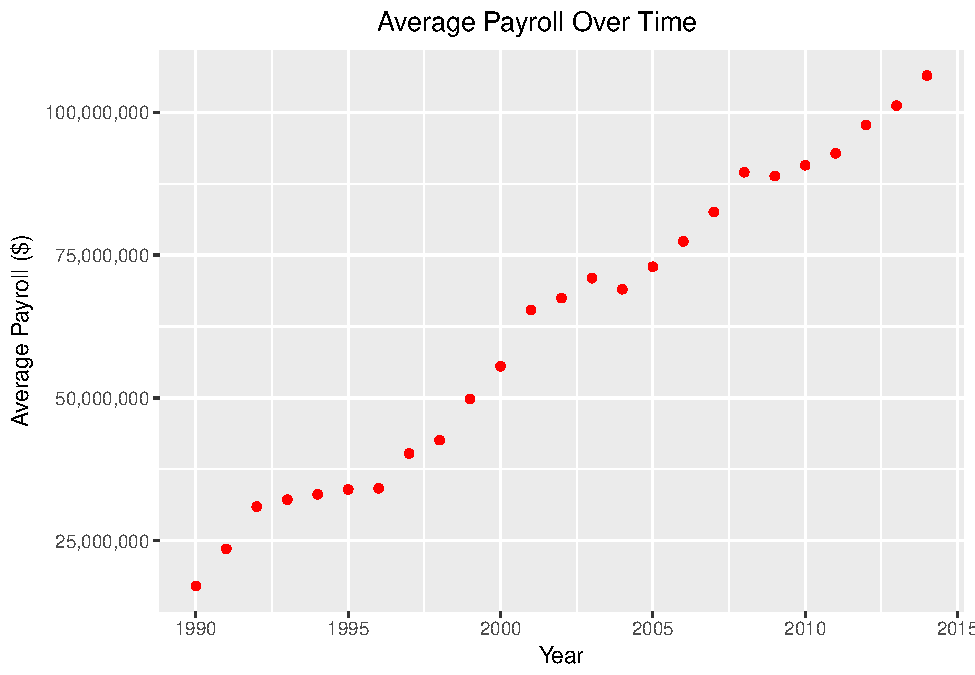
\includegraphics{p2_files/figure-latex/unnamed-chunk-5-1.pdf}

\textbf{Plot 2: Team Payrolls Over Time}

\begin{Shaded}
\begin{Highlighting}[]
\NormalTok{payroll_tab }\OperatorTok
\StringTok{  }\KeywordTok{filter}\NormalTok{(yearID }\OperatorTok{>=}\StringTok{ }\DecValTok{1990}\NormalTok{, yearID }\OperatorTok{<=}\StringTok{ }\DecValTok{2014}\NormalTok{) }\OperatorTok
\StringTok{  }\KeywordTok{ggplot}\NormalTok{(}\KeywordTok{aes}\NormalTok{(}\DataTypeTok{x =}\NormalTok{ yearID, }\DataTypeTok{y =}\NormalTok{ payroll)) }\OperatorTok{+}
\StringTok{    }\KeywordTok{facet_wrap}\NormalTok{(}\OperatorTok{~}\NormalTok{teamID) }\OperatorTok{+}
\StringTok{    }\KeywordTok{geom_line}\NormalTok{(}\DataTypeTok{color =} \StringTok{"red"}\NormalTok{) }\OperatorTok{+}
\StringTok{    }\KeywordTok{scale_y_continuous}\NormalTok{(}\DataTypeTok{labels =}\NormalTok{ comma) }\OperatorTok{+}\StringTok{ }
\StringTok{    }\KeywordTok{labs}\NormalTok{(}\DataTypeTok{title =} \StringTok{"Team Payrolls Over Time"}\NormalTok{, }\DataTypeTok{x =} \StringTok{"Year"}\NormalTok{, }\DataTypeTok{y =} \StringTok{"Total Payroll ($)"}\NormalTok{) }\OperatorTok{+}
\StringTok{    }\KeywordTok{theme}\NormalTok{(}\DataTypeTok{text =} \KeywordTok{element_text}\NormalTok{(}\DataTypeTok{size =} \FloatTok{6.5}\NormalTok{), }\DataTypeTok{plot.title =} \KeywordTok{element_text}\NormalTok{(}\DataTypeTok{hjust =} \FloatTok{0.5}\NormalTok{))}
\end{Highlighting}
\end{Shaded}

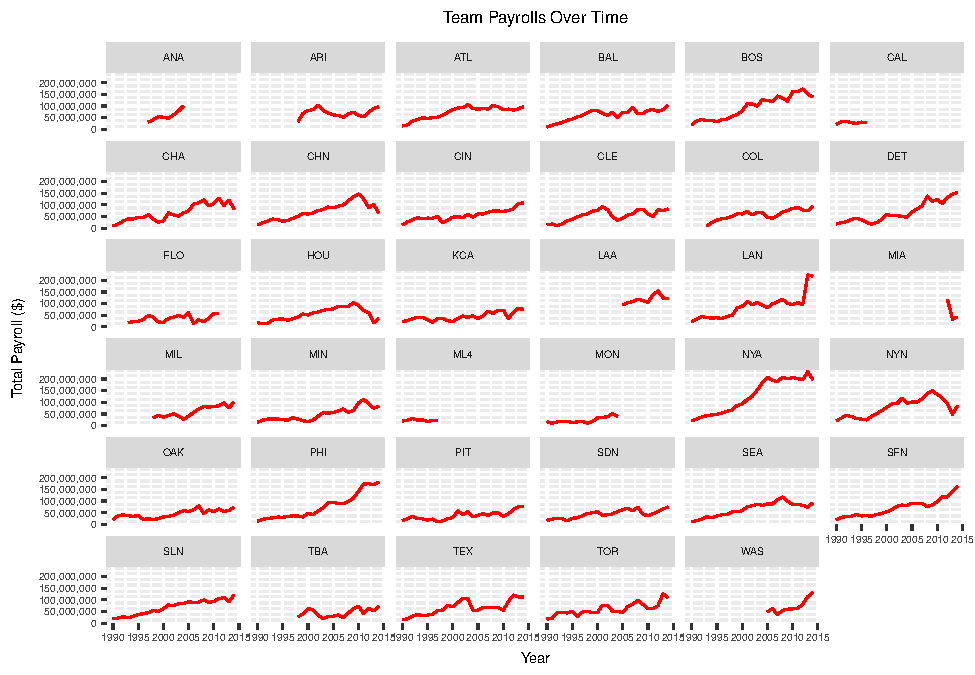
\includegraphics{p2_files/figure-latex/unnamed-chunk-6-1.pdf}

\emph{\textbf{Question 1:} What statements can you make about the
distribution of payrolls across time based on these plots? Remember you
can make statements in terms of central tendency, spread, etc.}

\begin{itemize}
\tightlist
\item
  Plot 1: Mean payroll has increased over time. (which makes sense
  economically)
\item
  Plot 2: It seems as if average payrolls of teams are increasing over
  time. (issue: spread and skew is difficult to see)
\end{itemize}

\emph{\textbf{Problem 3:} Write code to produce a plot(s) that
specifically show at least one of the statements you made in Question
1.}

\textbf{Plot 3: Trend of All Team Payrolls Over Time}

\begin{Shaded}
\begin{Highlighting}[]
\CommentTok{# Put all of these on one large plot}
\NormalTok{payroll_tab }\OperatorTok
\StringTok{  }\KeywordTok{filter}\NormalTok{(yearID }\OperatorTok{>=}\StringTok{ }\DecValTok{1990}\NormalTok{, yearID }\OperatorTok{<=}\StringTok{ }\DecValTok{2014}\NormalTok{) }\OperatorTok
\StringTok{    }\KeywordTok{ggplot}\NormalTok{(}\KeywordTok{aes}\NormalTok{(}\DataTypeTok{x =}\NormalTok{ yearID, }\DataTypeTok{y =}\NormalTok{ payroll)) }\OperatorTok{+}
\StringTok{      }\KeywordTok{geom_point}\NormalTok{(}\DataTypeTok{color =} \StringTok{"red"}\NormalTok{) }\OperatorTok{+}
\StringTok{      }\KeywordTok{geom_smooth}\NormalTok{(}\DataTypeTok{method =} \StringTok{"lm"}\NormalTok{) }\OperatorTok{+}
\StringTok{      }\KeywordTok{scale_y_continuous}\NormalTok{(}\DataTypeTok{labels =}\NormalTok{ comma) }\OperatorTok{+}\StringTok{ }
\StringTok{      }\KeywordTok{labs}\NormalTok{(}\DataTypeTok{title =} \StringTok{"Trend of All Team Payrolls Over Time"}\NormalTok{, }\DataTypeTok{x =} \StringTok{"Year"}\NormalTok{, }\DataTypeTok{y =} \StringTok{"Total Payroll ($)"}\NormalTok{) }\OperatorTok{+}
\StringTok{      }\KeywordTok{theme}\NormalTok{(}\DataTypeTok{plot.title =} \KeywordTok{element_text}\NormalTok{(}\DataTypeTok{hjust =} \FloatTok{0.4}\NormalTok{))}
\end{Highlighting}
\end{Shaded}

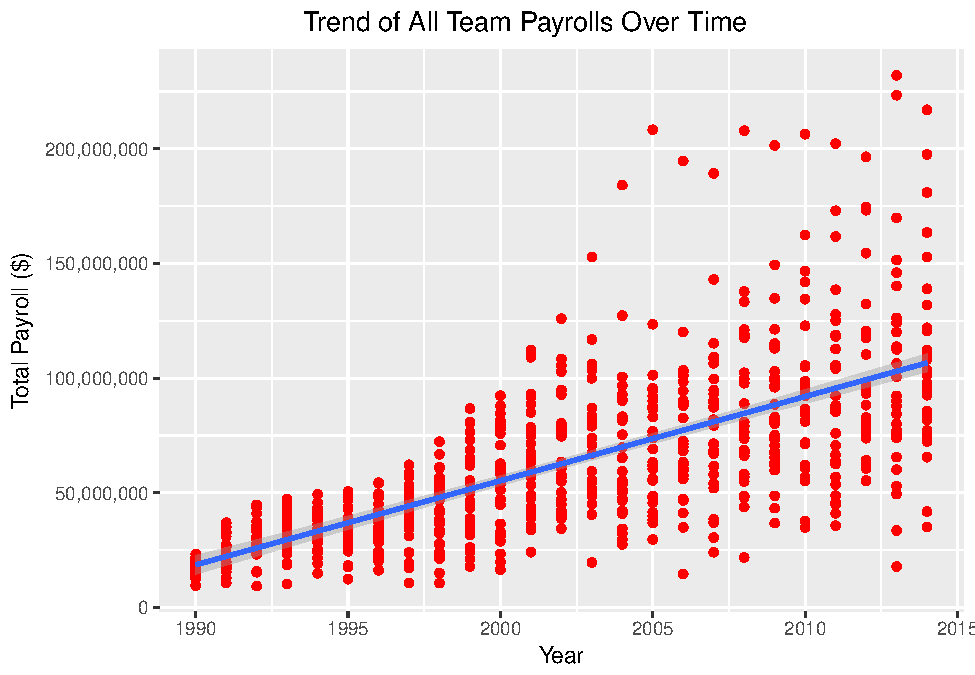
\includegraphics{p2_files/figure-latex/unnamed-chunk-7-1.pdf}

By combining the data from Plot 2 into one plot, we can definitively see
that average payrolls of teams are increasing over time. Spread and skew
are also visible now. The spread of team payrolls is increasing across
most, if not all teams over time. There is also some skew among payrolls
since the value of these teams change over time, affecting the salaries
the teams are able to pay their athletes.


\end{document}
